\documentclass[10pt]{article}
\usepackage[a4paper,margin=2cm]{geometry}
\usepackage{booktabs,longtable,amsmath,amssymb,graphicx,pdfpages,caption,lscape}
\captionsetup{font=small,labelfont=bf}
\title{\bfseries CL inflow fits with a virial window for the SPARC category-C galaxies:\\ detection, model selection, fit quality and robustness}
\author{Automated analysis for E.P.J.\ de Haas}\date{}
\begin{document}\maketitle
\section*{Summary}
Category C contains the 41 SPARC galaxies whose single-Lagrangian (single-L) residuals show a significant $-+-$ wave: the data rise above the CL curve at intermediate radii and fall below it further out. For all of them we fitted the CL inflow model extended with a virial window, as introduced in de Haas (2026) [1] and in the CL field paper [2]. Beyond a radius $r_v$ the orbital speed gains a Newtonian component of strength $p$. The window is accepted in 29 galaxies ($\Delta\mathrm{BIC}<-6$ relative to single-L); in 12 the wave is too weak and single-L is kept. In 26 of the accepted galaxies the window is a \emph{descent} ($p>2$): beyond $r_v$, $v^2$ falls as $GM_N/r$ onto a floor $A$. For these, median $\chi^2_\nu$ falls from 4.28 to 1.01, RMS$_\mathrm{rel}$ from 0.117 to 0.073, and the window radius, floor and descent mass are determined to 9\%, 6\% and 23\% (medians). The window is preferred over the two-Lagrangian alternative in every accepted galaxy, and a free gauge offset is never required. The descent galaxies are early and intermediate spirals (Sab--Sc), complementary to the late-type nested-spiral galaxies of category B. Residual structure persists in 18 of 26, and 7 remain at $\chi^2_\nu>2$; these are bulge-dominated curves with very small errors, where the inner rise and peak need further regions.

\section{Models}
\paragraph{Single-L.} The CL inflow curve of [2] (Eqs.~17--18; see also [1, Eqs.~4--5] and [3]), with $X=\sqrt{2GM/R}-H_zR$ and $Y(r)=\sqrt{2GM/r}-H_zr$:
\begin{equation*}v^2=\tfrac12X^2r^2/R^2\ (r\le R),\qquad v^2=\tfrac32X^2-Y(r)^2\ (r>R),\qquad H_z=2.2\times10^{-18}\,\mathrm{s^{-1}}.\end{equation*}
\paragraph{CL + virial window (VW).} Following [1, Eq.~6] and [2, Eq.~19], beyond $r_v$:
\begin{equation*}v^2(r)=\tfrac32X^2-Y(r)^2+p\Bigl[\tfrac12Y(r)^2-\Phi_p\Bigr],\qquad r\ge r_v.\end{equation*}
Two choices differ from [1], where $r_v$ is set by inspection and $\Phi_p$ is free. Here $r_v$ is fitted, and $\Phi_p=\tfrac12Y(r_v)^2$ makes $v^2$ continuous at $r_v$; leaving $\Phi_p$ free (model VWf, $k=5$) is tested separately. For $H_z\to0$ the window reads
\begin{equation*}v^2=A+\frac{GM_N}{r},\qquad A=\frac{3GM}{R}-\frac{pGM}{r_v},\qquad M_N=(p-2)\,M,\end{equation*}
so $p>2$ gives a Keplerian descent of mass $M_N$ onto the floor $A$, $0<p<2$ a flattening, $p<0$ an additional rise, and $p=3$ the pure Kepler term of the inner mass $M$. Because $p$ and $M$ become degenerate when the descent dominates, the fit is parametrised by $(M,R,r_v,M_N)$, which are also the measured quantities. This descent behaviour was first noticed in earlier spreadsheet fits as solutions with formally negative $(M,R)$, which have exactly the $A+B/r$ form; the window replaces them with positive parameters valid for $H_z\neq0$.
\paragraph{Alternatives.} Two-L ([2, Eqs.~24--26]; $k=4$, the same parameter count as VW), and VWf ($k=5$).
\paragraph{Selection and uncertainties.} The window is accepted when $\Delta\mathrm{BIC}=\mathrm{BIC_{VW}}-\mathrm{BIC_S}<-6$, and assigned to two-L instead if two-L has lower BIC by more than 2. Uncertainties come from five sources. (1) Statistical: local covariance; $A$ by linear propagation. (2) $r_v$: since $\partial v^2/\partial r$ is discontinuous at $r_v$, $\chi^2(r_v)$ changes slope at each data radius, so a profile-likelihood interval ($\Delta\chi^2\le1$, 80 grid values, other parameters refitted) is used. (3) Jackknife: leave-one-out. (4) Systematic: distance $+\delta D$ and inclination $+\delta i$ refits. (5) $H_z=0$ refit. The profile scan also served as a global check of the optimum; it found a better solution for NGC 6674, which was adopted.
\paragraph{Grades (descent windows).} \textbf{I}: $R$, $r_v$, $M_N$ and $A$ all within 30\%, at least 3 points on each side of $r_v$, jackknife scatter $\le30\%$. \textbf{II}: $A$ within 10\% and $M_N$ within 50\%. \textbf{III}: otherwise. \textbf{M} flag: $\chi^2_\nu>2$ after the window.

\section{Model selection outcome}
\begin{table}[h]\centering\small\caption{Category-C outcome.}\begin{tabular}{lrl}\toprule Outcome & $N$ & Galaxies\\\midrule
Descent window, grade I & 7 & \parbox[t]{10.5cm}{\raggedright NGC2903, NGC3198, NGC3992, NGC4100, NGC5055, UGC02953, UGC05253}\\
Descent window, grade II & 7 & \parbox[t]{10.5cm}{\raggedright NGC4157, NGC5907, NGC6503, NGC6674, NGC7331, UGC03205, UGC08699}\\
Descent window, grade III & 12 & \parbox[t]{10.5cm}{\raggedright NGC0891, NGC3521, NGC4088, NGC4217, NGC5033, NGC5371, NGC5985, UGC02916, UGC05986, UGC11455, UGC11914, UGC12506}\\
Flattening window ($0<p<2$) & 2 & \parbox[t]{10.5cm}{\raggedright ESO563--G021, IC4202}\\
Rising window ($p<0$) & 1 & \parbox[t]{10.5cm}{\raggedright NGC6946}\\
Single-L kept & 12 & \parbox[t]{10.5cm}{\raggedright F568--V1, NGC1705, NGC2366, NGC3769, NGC4183, NGC4559, UGC01230, UGC04305, UGC05721, UGC06983, UGC08490, UGC09037}\\
\bottomrule\end{tabular}\\[2pt]{\footnotesize Galaxies with $\chi^2_\nu>2$ after the window (flag M): NGC2903, NGC5055, NGC5371, NGC5907, NGC6674, NGC6946, UGC02953, UGC11455.}\end{table}
\textbf{Window versus two-L.} With the same number of parameters, the window beats the two-Lagrangian model in every accepted galaxy (smallest $\mathrm{BIC_{2L}-BIC_{VW}}$ = +2.2, median +43). A two-L reset produces an upward step and cannot follow a $1/r$ descent, so category C is genuinely different from category B. \textbf{Free gauge.} Leaving $\Phi_p$ free never helps ($\Delta\mathrm{BIC_{VWf-VW}}\ge-1.0$), so the data show no step at $r_v$ and the continuous gauge is adequate. \textbf{Single-L kept.} The 12 rejected galaxies already have small single-L $\chi^2_\nu$ (median 0.48) and are mostly late types; their $-+-$ wave lies within the SPARC errors. \textbf{Other windows.} ESO563-G021 and IC 4202 need an outer \emph{flattening} ($p\approx1.7$), and NGC 6946 needs an extra \emph{rise} ($p<0$, with two-L only $+2.2$ behind). That makes NGC 6946 a borderline case between categories B and C.
\begin{figure}[h]\centering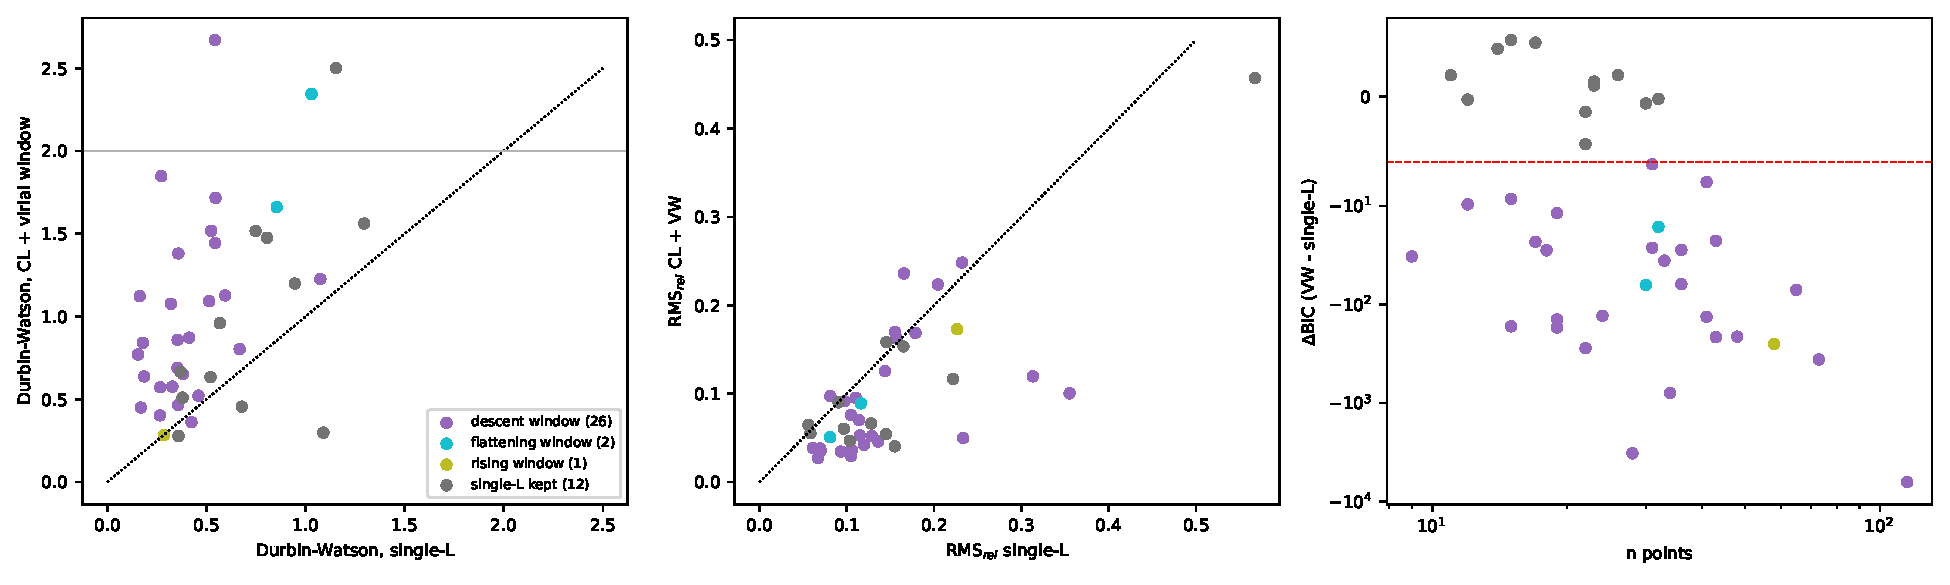
\includegraphics[width=\textwidth]{catC_fig_quality.pdf}\caption{Left: Durbin--Watson statistic before and after the window. Middle: relative RMS in $v^2$. Right: $\Delta$BIC (VW $-$ single-L) versus $n$; acceptance threshold $-6$. Colours: descent (purple), flattening (cyan), rising (olive), single-L kept (grey).}\end{figure}
\section{Fit quality of the descent windows}
\begin{table}[h]\centering\small\caption{Descent-window galaxies: fit-quality statistics (medians, single-L $\to$ CL + virial window).}\begin{tabular}{lrrr}\toprule & Grade I & Grade II & Grade III\\\midrule
$\chi^2_\nu$ & 6.72 $\to$ 0.75 & 4.58 $\to$ 1.03 & 2.21 $\to$ 1.02\\
RMS$_\mathrm{rel}$ & 0.232 $\to$ 0.100 & 0.129 $\to$ 0.052 & 0.108 $\to$ 0.084\\
Durbin--Watson & 0.33 $\to$ 0.77 & 0.36 $\to$ 0.87 & 0.37 $\to$ 0.94\\
$p_\mathrm{runs}<0.05$ after window & 6/7 & 5/7 & 7/12\\
$\Delta$BIC (median) & -361 & -133 & -25\\
$n$ (median) & 34 & 31 & 26\\
\bottomrule\end{tabular}\end{table}
The window removes the dominant $-+-$ pattern in all descent galaxies. The median Durbin--Watson statistic rises from 0.36 to 0.85, and the residual sign pattern loses its long runs (atlas). Residual structure is not fully removed in 18 galaxies. Unlike categories A and B, category C contains many high-precision, bulge-dominated curves (median $n=31$, 20 of 26 Q=1). There small, coherent deviations near the inner peak become significant: 10 galaxies have at least one residual beyond $3\sigma$, and Shapiro--Wilk rejects normality in 9. The SPARC errors are again conservative on average (5 galaxies with $P(\chi^2\le\chi^2_\mathrm{obs})<0.01$), so $\chi^2_\nu<1$ is not unusual. The flag-M galaxies (NGC2903, NGC5055, NGC5371, NGC5907, NGC6674, NGC6946, UGC02953, UGC11455) are improved by factors of 2 to 30 in $\chi^2$, but their inner bulge region and peak are not described by a single CL bulge. They are the natural targets for a bulge Lagrangian plus disk Lagrangian with a window, or for the two-window scheme of [1, Eqs.~5--7].
\section{Parameter determination}
Median relative uncertainties for the descent windows are: $R$ 14\%, $r_v$ 9\% (profile), $M_N$ 23\%, $A$ 5.8\%, and $M$ 16\%. The floor $A$ and the window radius are the best-determined quantities. The parametrisation by $M_N$ removes the $p$--$M$ degeneracy (median $\rho(M,M_N)=0.00$). The virial strength $p=2+M_N/M$ is then a derived quantity, and it becomes very large where $M$ is small: in NGC 891, NGC 5033, NGC 6674, UGC 2916 and UGC 5253 the inner CL bulge shrinks and the curve is a compact central mass plus Keplerian descent. $p$ ranges over 3.8--61 (16--84\%, median 7.1), and 8 galaxies have $p\le5$. The pure Kepler case $p=3$ is therefore one end of a broad distribution, not a universal value.

\paragraph{The $r_v$ likelihood.} Fig.~2 shows that $\chi^2(r_v)$ has a well-defined minimum in most galaxies, kinked at the data radii. Because $v^2$ is continuous at $r_v$, the profile is smoother than the $R_2$ profile of the two-L model, and $r_v$ is localised to within one or two point spacings.

\paragraph{Systematics, jackknife, $H_z$.} Distance and inclination systematics are comparable to or larger than the statistical errors (median sys/stat 1.7 for $r_v$, 0.9 for $A$, 0.5 for $M_N$). Leave-one-out scatter stays below 30\% for grade I. Setting $H_z=0$ changes the parameters by at most about 12\% except in NGC 5033 and UGC 2916, where the inner $R$ is poorly constrained and the solution moves along the $M$--$R$ degeneracy.
\begin{figure}[h]\centering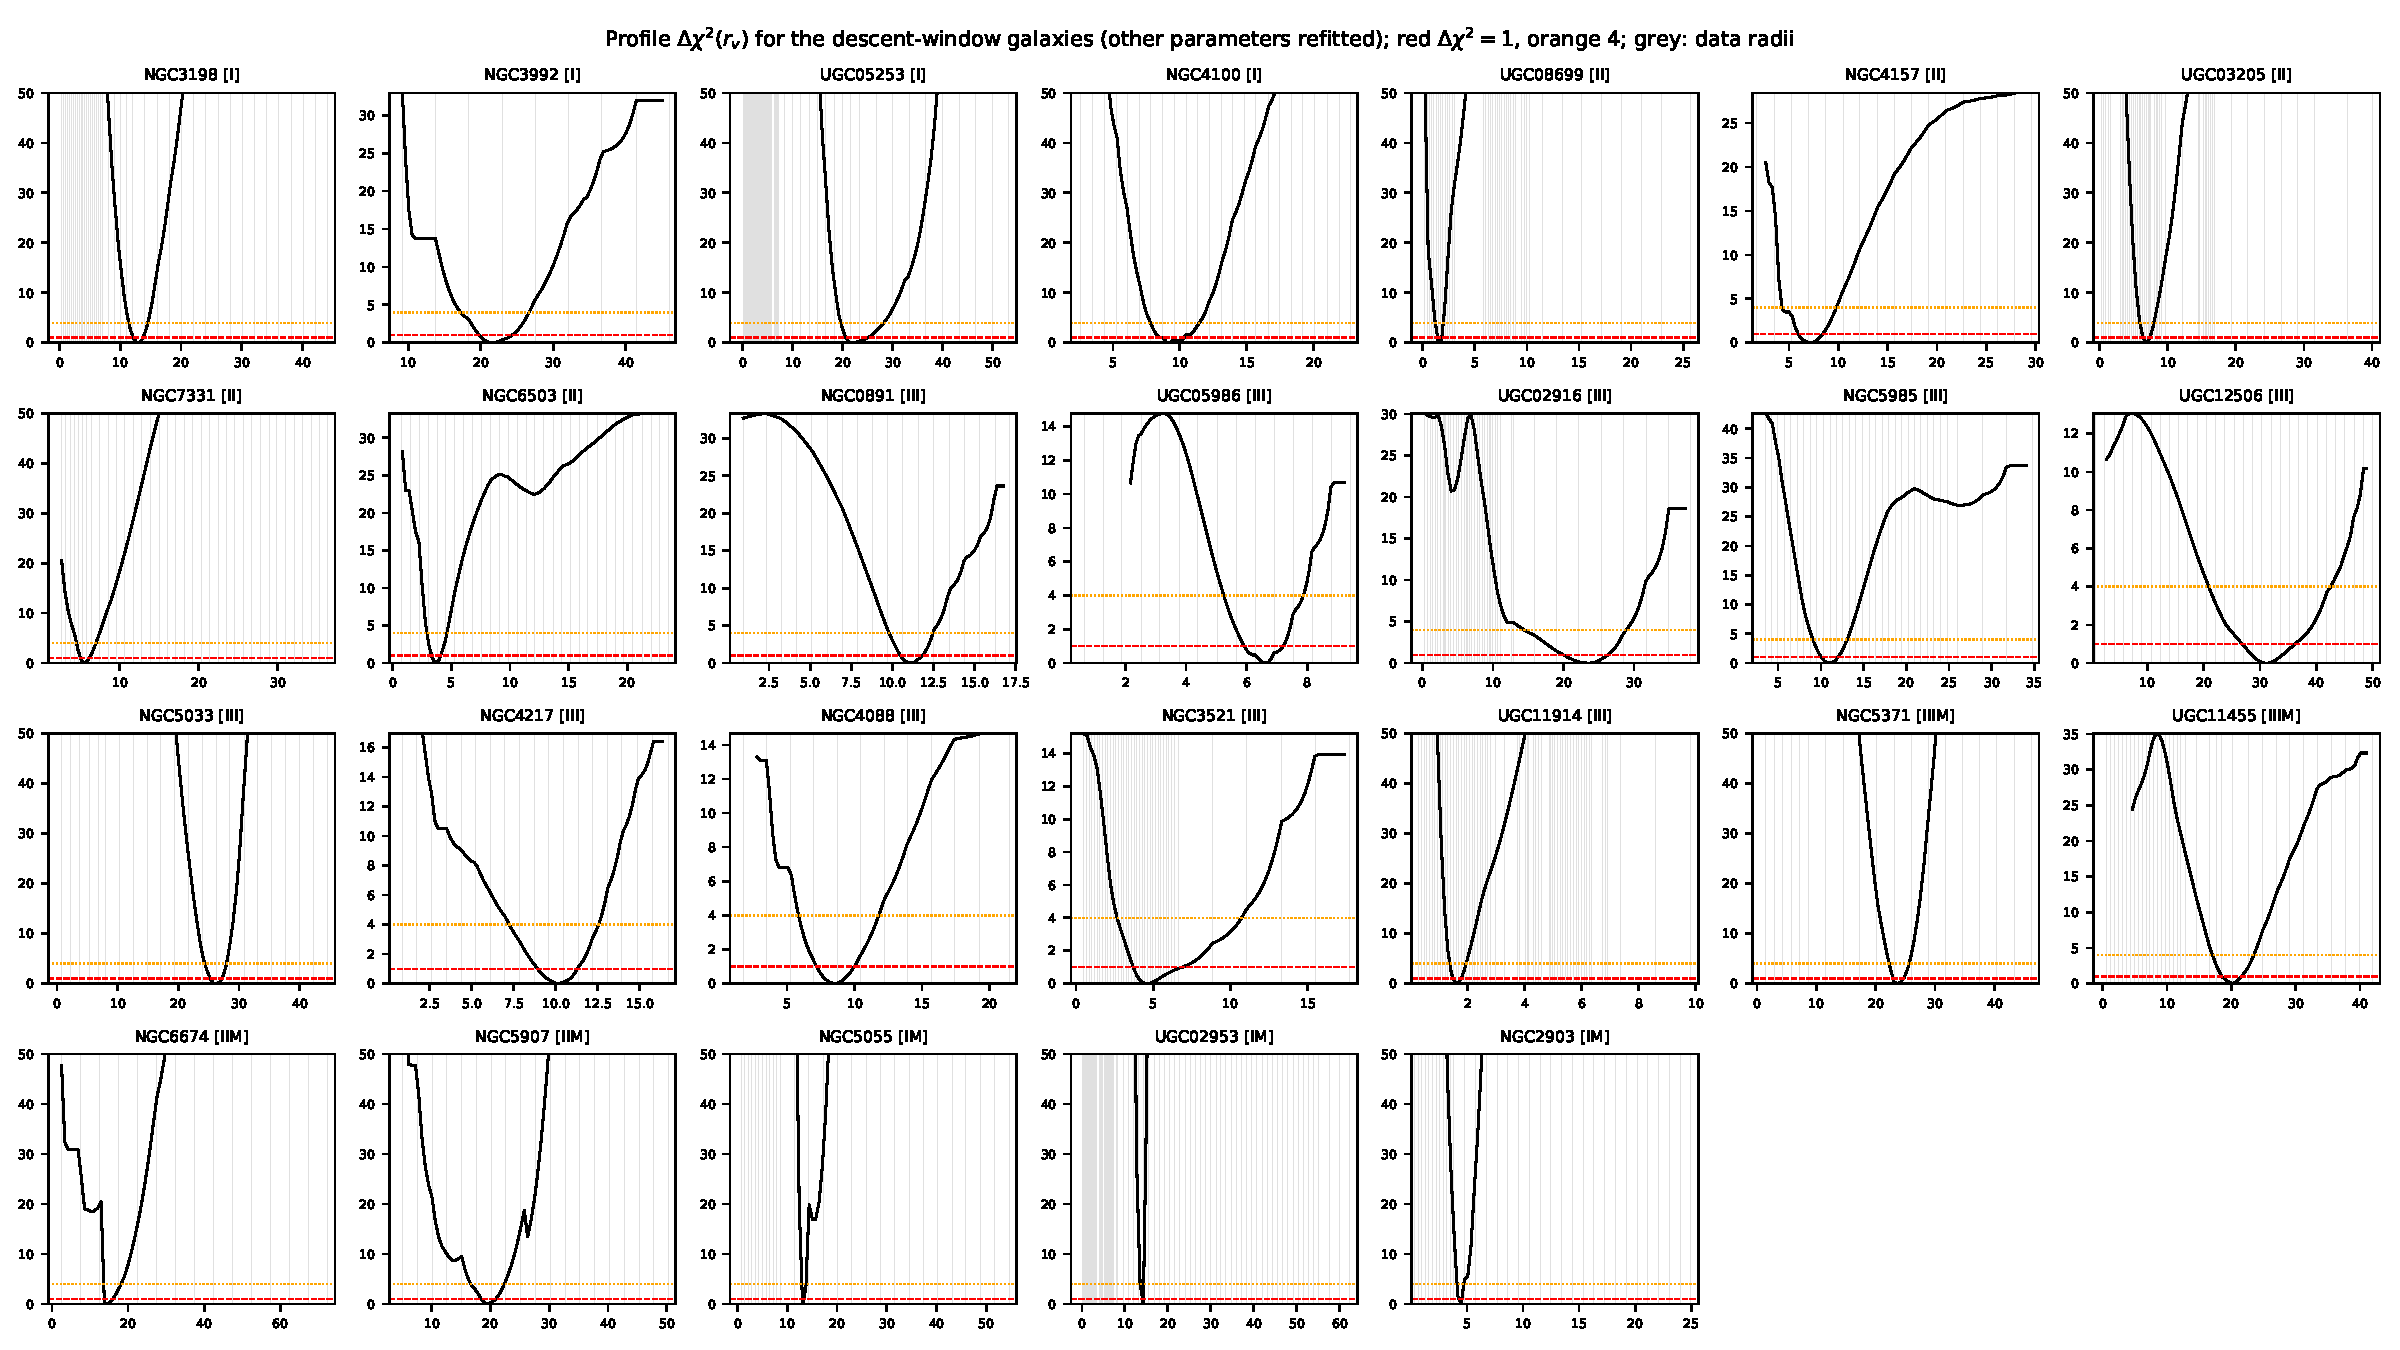
\includegraphics[width=\textwidth]{catC_fig_profiles.pdf}\caption{Profile $\Delta\chi^2(r_v)$ for the descent-window galaxies; grey lines are the data radii.}\end{figure}
\section{Physical consistency}
\begin{itemize}\itemsep0pt
\item \textbf{Window radius.} $r_v$ = 4.6--21.7\,kpc (median 11.1), $r_v/R_\mathrm{disk}$ = 3.4 (16--84\%: 1.8--4.2; Spearman $\rho$ = 0.76). The descent sets in at 2--4 disk scale lengths, beyond the rotation-curve peak.
\item \textbf{Floor.} $\sqrt{A}$ tracks SPARC $V_\mathrm{flat}$ ($r$ = 0.92), with $\sqrt{A}/V_\mathrm{flat}$ = 0.92. The floor is the asymptotic speed that the descent approaches; $V_\mathrm{flat}$, measured over the last points, lies slightly above it because the descent is not yet complete.
\item \textbf{Descent mass.} $M_N/M_\mathrm{bar}$ = 0.58 (16--84\%: 0.14--1.42; $r$ = 0.63 in log). For the 13 galaxies with a photometric bulge, $M_N$ is 2.8 times the bulge stellar mass ($\Upsilon_\mathrm{bulge}=0.7$; 16--84\%: 0.8--8.8). The Keplerian descent mass is therefore of the order of the baryonic mass inside the peak, consistent with the reading in [1] that the window matter orbits Newtonially with respect to the inflowing metric.
\item \textbf{Morphology.} The descent windows are early and intermediate spirals (Sab 6, Sb 6, Sbc 7, Sc 3, Scd 3, Sm 1), with 20 of 26 Q=1. The single-L-kept galaxies are mostly Scd--BCD. Together with category B (late-type nested spirals), this gives a clean morphological split. Bulge-dominated galaxies show a Keplerian descent window; bulgeless late types show a Lagrangian reset.
\end{itemize}
\begin{figure}[h]\centering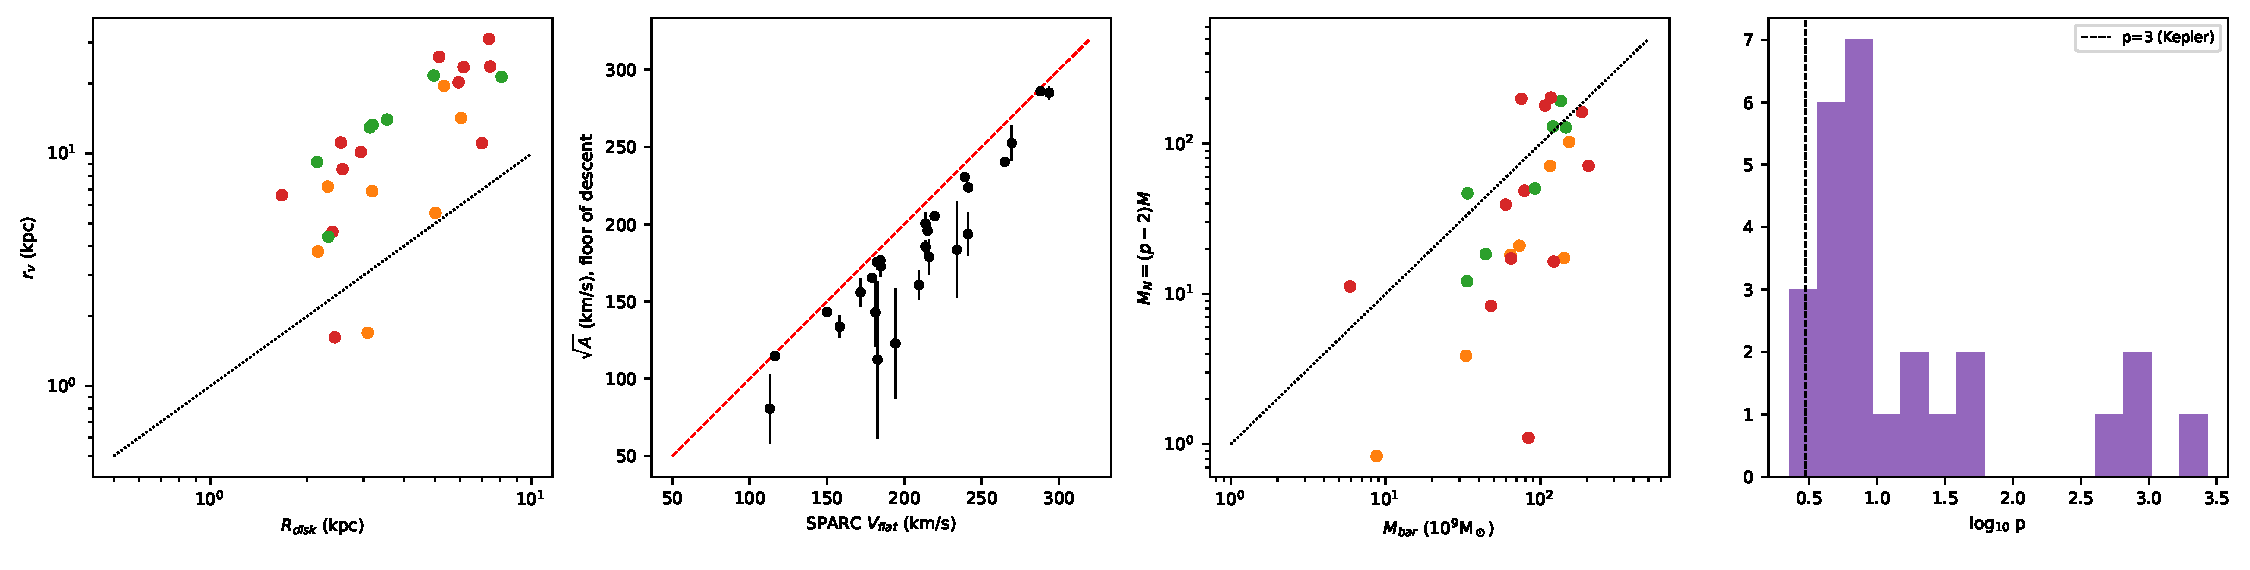
\includegraphics[width=\textwidth]{catC_fig_physics.pdf}\caption{Descent windows. Left to right: $r_v$ versus $R_\mathrm{disk}$; floor $\sqrt A$ versus SPARC $V_\mathrm{flat}$; descent mass $M_N$ versus $M_\mathrm{bar}$; distribution of the virial strength $p$ (dashed: pure Kepler $p=3$). Colours: grade I green, II orange, III red.}\end{figure}
\section{Assessment}
\textbf{The descent is a robust, recurring feature.} The CL + virial window of [1,2], with $r_v$ fitted and a continuous gauge, describes 26 of the 41 category-C galaxies far better than single-L ($\Delta$BIC from -6 to -6318). It is always preferred over a two-Lagrangian reset and needs no free gauge. Its measured quantities, the window radius $r_v$, the floor $A$ and the Keplerian descent mass $M_N$, are well determined and match independent photometric and kinematic scales.

\textbf{Grades.} Grade I (NGC2903, NGC3198, NGC3992, NGC4100, NGC5055, UGC02953, UGC05253) is the robust core. Grade II (NGC4157, NGC5907, NGC6503, NGC6674, NGC7331, UGC03205, UGC08699) has a well-determined floor and window but a less certain descent mass. Grade III (NGC0891, NGC3521, NGC4088, NGC4217, NGC5033, NGC5371, NGC5985, UGC02916, UGC05986, UGC11455, UGC11914, UGC12506) has a weakly determined descent mass ($>50$\%) or floor ($>10$\%), mostly because only a few points lie in the window, the descent is shallow ($p$ close to 2), or the inner radius is unconstrained.

\textbf{Limits.} (i) The inner bulge region of the most massive, best-measured spirals is not captured by a single CL bulge, which leaves residual structure in about two thirds of the descent galaxies and $\chi^2_\nu>2$ in eight. (ii) $p$ is not a robust quantity when the inner mass is small; $M_N$ and $A$ should be reported instead. (iii) The window has no outer end here. The two-window scheme of [1] (window strengths $p$, $q$) is the natural next refinement for the flag-M galaxies, together with an explicit bulge component.

\section*{References}
\small
[1] E.P.J.\ de Haas (2026), From Rotation Curves to Cosmic Time: Probing High-Redshift Expansion through Nested Spiral Dynamics, \emph{J.\ High Energy Phys.\ Grav.\ Cosmol.} 12, 334--367, doi:10.4236/jhepgc.2026.121022 (virial term Eq.~3; multi-region virial model Eqs.~5--7).\par
[2] E.P.J.\ de Haas, Galactic Rotation Curves and the Constant--Lagrangian Field: Empirical Tests within the $Q_g$ Rotor Framework (manuscript; single-L Eqs.~17--18, virial term Eq.~19, two-L Eqs.~24--26).\par
[3] E.P.J.\ de Haas, The Role of the Hubble Parameter in Galactic Rotation Curves and Spiral Morphology (manuscript).\par
[4] F.\ Lelli, S.S.\ McGaugh, J.M.\ Schombert (2016), SPARC, \emph{AJ} 152, 157.

\clearpage\begin{landscape}{\scriptsize\setlength{\tabcolsep}{3pt}
\begin{longtable}{lllrrrrrrrrrll}
\caption{All category-C galaxies: single-L, CL + virial window (VW), two-L and VWf comparison.}\\\toprule
Galaxy & Type & Q & $n$ & $\chi^2_{\nu,S}$ & RMS$_S$ & $p_\mathrm{runs,S}$ & $\chi^2_{\nu,VW}$ & $\Delta$BIC$_{VW}$ & BIC$_{2L}-$BIC$_{VW}$ & BIC$_{VWf}-$BIC$_{VW}$ & $p$ & Outcome & Grade\\\midrule\endfirsthead
\toprule Galaxy & Type & Q & $n$ & $\chi^2_{\nu,S}$ & RMS$_S$ & $p_\mathrm{runs,S}$ & $\chi^2_{\nu,VW}$ & $\Delta$BIC$_{VW}$ & BIC$_{2L}-$BIC$_{VW}$ & BIC$_{VWf}-$BIC$_{VW}$ & $p$ & Outcome & Grade\\\midrule\endhead\bottomrule\endfoot
UGC02953 & Sab & 2 & 115 & 68.64 & 0.232 & 1.2e-24 & 12.87 & -6317.8 & +5081.6 & +4.7 & 35.8 & descent window & IM\\
NGC5055 & Sbc & 1 & 28 & 128.68 & 0.313 & 2.9e-06 & 4.36 & -3234.6 & +732.1 & +3.3 & 14.5 & descent window & IM\\
NGC2903 & Sbc & 1 & 34 & 26.86 & 0.355 & 1.0e-07 & 2.10 & -789.5 & +543.6 & +3.5 & 5.19 & descent window & IM\\
UGC05253 & Sab & 2 & 73 & 5.54 & 0.093 & 3.0e-15 & 0.35 & -360.7 & +10.8 & +1.1 & 496 & descent window & I\\
NGC5033 & Sc & 1 & 22 & 15.11 & 0.119 & 5.3e-05 & 1.04 & -277.3 & +84.2 & -1.0 & 2.68e+03 & descent window & III\\
NGC6946 & Scd & 1 & 58 & 9.71 & 0.226 & 8.4e-09 & 5.27 & -251.4 & +2.2 & +4.1 & -284 & rising window & --\\
NGC3198 & Sc & 1 & 43 & 6.13 & 0.204 & 5.7e-09 & 0.75 & -214.2 & +219.2 & +3.8 & 3.8 & descent window & I\\
UGC03205 & Sab & 1 & 48 & 5.93 & 0.179 & 1.2e-07 & 1.21 & -211.8 & +218.1 & +3.4 & 6.36 & descent window & II\\
NGC5371 & Sbc & 1 & 19 & 14.64 & 0.110 & 2.5e-04 & 4.79 & -171.2 & +89.3 & +2.9 & 40.2 & descent window & IIIM\\
NGC6674 & Sb & 1 & 15 & 16.38 & 0.165 & 3.1e-02 & 3.74 & -166.4 & +172.2 & +21.2 & 818 & descent window & IIM\\
NGC5907 & Sc & 1 & 19 & 10.88 & 0.070 & 2.1e-04 & 2.50 & -141.6 & +147.9 & +2.9 & 15.2 & descent window & IIM\\
UGC08699 & Sab & 2 & 41 & 4.58 & 0.114 & 1.2e-07 & 1.03 & -133.3 & +98.5 & +3.7 & 7.8 & descent window & II\\
NGC4100 & Sbc & 1 & 24 & 6.72 & 0.233 & 1.6e-05 & 0.57 & -130.0 & +64.5 & +3.2 & 6.28 & descent window & I\\
UGC11914 & Sab & 1 & 65 & 2.22 & 0.081 & 9.0e-14 & 0.99 & -70.9 & +79.3 & +4.2 & 2.27 & descent window & III\\
ESO563--G021 & Sbc & 1 & 30 & 3.38 & 0.116 & 4.2e-06 & 0.94 & -63.3 & +29.0 & +3.4 & 1.76 & flattening window & --\\
NGC7331 & Sb & 1 & 36 & 2.70 & 0.067 & 4.0e-04 & 0.71 & -62.2 & +70.2 & +3.6 & 3.96 & descent window & II\\
NGC5985 & Sb & 1 & 33 & 2.20 & 0.069 & 1.4e-03 & 0.88 & -35.9 & +42.9 & +3.0 & 2.63 & descent window & III\\
NGC3992 & Sbc & 1 & 9 & 5.62 & 0.105 & 3.9e-02 & 0.48 & -32.5 & +22.8 & +2.2 & 9.26 & descent window & I\\
NGC0891 & Sb & 1 & 18 & 3.06 & 0.097 & 1.9e-03 & 1.06 & -28.2 & +54.4 & +2.5 & 61.5 & descent window & III\\
UGC11455 & Scd & 1 & 36 & 3.97 & 0.155 & 2.0e-07 & 3.12 & -28.0 & +21.2 & +3.5 & 4.15 & descent window & IIIM\\
NGC6503 & Scd & 1 & 31 & 1.92 & 0.136 & 3.9e-03 & 0.82 & -26.5 & +33.4 & -0.8 & 2.78 & descent window & II\\
NGC4157 & Sb & 1 & 17 & 2.10 & 0.129 & 9.9e-04 & 0.21 & -23.1 & +26.6 & +2.8 & 3.68 & descent window & II\\
UGC02916 & Sab & 2 & 43 & 2.48 & 0.115 & 1.1e-06 & 1.84 & -22.5 & +19.0 & +3.8 & 848 & descent window & III\\
IC4202 & Sbc & 1 & 32 & 1.31 & 0.081 & 2.1e-02 & 0.57 & -16.3 & +10.9 & +3.5 & 1.65 & flattening window & --\\
NGC4217 & Sb & 1 & 19 & 1.11 & 0.106 & 2.1e-04 & 0.08 & -11.8 & +8.8 & +2.9 & 7.77 & descent window & III\\
NGC4088 & Sbc & 1 & 12 & 1.81 & 0.105 & 8.3e-03 & 0.40 & -9.9 & +10.0 & +2.5 & 3.94 & descent window & III\\
UGC05986 & Sm & 2 & 15 & 2.15 & 0.144 & 8.1e-03 & 1.20 & -9.4 & +7.3 & +2.7 & 5.84 & descent window & III\\
NGC3521 & Sbc & 1 & 41 & 0.45 & 0.061 & 2.9e-06 & 0.07 & -7.8 & +10.5 & +3.7 & 6.03 & descent window & III\\
UGC12506 & Scd & 2 & 31 & 0.71 & 0.157 & 2.6e-06 & 0.28 & -6.2 & +6.0 & +3.4 & 16.7 & descent window & III\\
UGC09037 & Scd & 2 & 22 & 0.86 & 0.091 & 2.7e-04 & 0.37 & -4.4 & +1.6 & +2.9 & -2.42 & single-L kept & --\\
UGC04305 & Im & 3 & 22 & 0.65 & 0.568 & 1.3e-03 & 0.30 & -1.4 & +4.2 & +3.1 & 2.2 & single-L kept & --\\
UGC08490 & Sm & 1 & 30 & 0.50 & 0.103 & 1.3e-04 & 0.25 & -0.6 & -0.1 & +3.4 & -4.95 & single-L kept & --\\
NGC3769 & Sb & 2 & 12 & 0.79 & 0.097 & 1.1e-02 & 0.32 & -0.3 & +4.0 & +2.3 & 4.79 & single-L kept & --\\
NGC4559 & Scd & 1 & 32 & 0.44 & 0.155 & 1.6e-06 & 0.21 & -0.2 & +0.0 & +3.5 & -12.7 & single-L kept & --\\
UGC05721 & Sd & 1 & 23 & 1.01 & 0.222 & 1.4e-04 & 0.84 & 1.0 & -0.1 & +3.1 & -12.3 & single-L kept & --\\
NGC4183 & Scd & 1 & 23 & 0.54 & 0.145 & 6.9e-04 & 0.34 & 1.3 & -0.1 & +3.1 & -8.64 & single-L kept & --\\
UGC01230 & Sm & 1 & 11 & 0.37 & 0.128 & 1.3e-02 & 0.07 & 1.9 & +0.8 & +2.4 & 2.14 & single-L kept & --\\
NGC2366 & Im & 3 & 26 & 0.47 & 0.165 & 3.2e-05 & 0.30 & 1.9 & +2.5 & +3.3 & 4.11 & single-L kept & --\\
NGC1705 & BCD & 3 & 14 & 0.15 & 0.058 & 4.9e-03 & 0.08 & 4.3 & +0.9 & +2.0 & 4.27 & single-L kept & --\\
UGC06983 & Scd & 1 & 17 & 0.32 & 0.056 & 1.4e-02 & 0.31 & 4.9 & -0.3 & +2.8 & -1.13 & single-L kept & --\\
F568--V1 & Sd & 1 & 15 & 0.08 & 0.145 & 8.1e-03 & 0.07 & 5.1 & +0.1 & +2.7 & 1.11 & single-L kept & --\\
\end{longtable}
\begin{longtable}{llrlllllllr}
\caption{Accepted windows: parameters. $R,r_v$ in kpc; $M,M_N$ in $10^9M_\odot$; $A$ in km$^2$s$^{-2}$. $R$, $M_N$, $A$: statistical $\pm$ systematic; $r_v$: profile $\Delta\chi^2\le1$ interval [systematic]. $n_\mathrm{in}/n_\mathrm{win}$: points before/after $r_v$.}\\\toprule
Galaxy & Grade & $n$ & $R$ & $M$ & $r_v$ & $M_N$ & $A$ & $p$ & $n_\mathrm{in}/n_\mathrm{win}$ & jk\\\midrule\endfirsthead
\toprule Galaxy & Grade & $n$ & $R$ & $M$ & $r_v$ & $M_N$ & $A$ & $p$ & $n_\mathrm{in}/n_\mathrm{win}$ & jk\\\midrule\endhead\bottomrule\endfoot
UGC05253 & I & 73 & $0.0561\pm0.015\pm0.013$ & $0.264\pm0.074$ & $21.4^{+3.1}_{-0.17}$ [5.4] & $130\pm11\pm41$ & $34364\pm1.6e+03\pm5.6e+03$ & 496 & 62/11 & 0.20\\
NGC3198 & I & 43 & $3\pm0.083\pm0.3$ & $6.74\pm0.27$ & $13^{+0.75}_{-0.78}$ [1.3] & $12.2\pm2.6\pm1.2$ & $20525\pm4.6e+02\pm5.9e+02$ & 3.8 & 27/16 & 0.19\\
NGC4100 & I & 24 & $2.82\pm0.22\pm0.39$ & $10.9\pm1.3$ & $9.19^{+1}_{-0.43}$ [1.3] & $46.7\pm5.9\pm6.5$ & $17860\pm1.9e+03\pm3.5e+02$ & 6.28 & 8/16 & 0.16\\
NGC3992 & I & 9 & $3.96\pm1.2\pm0.38$ & $26.5\pm9.9$ & $21.7^{+2.5}_{-1.6}$ [2.1] & $193\pm40\pm20$ & $37508\pm5.5e+03\pm1.6e+03$ & 9.26 & 3/6 & 0.09\\
UGC03205 & II & 48 & $1.01\pm0.074\pm0.2$ & $4.81\pm0.44$ & $6.89^{+0.42}_{-0.06}$ [1.4] & $21\pm2.5\pm4.3$ & $42131\pm6e+02\pm2.2e+03$ & 6.36 & 19/29 & 0.35\\
UGC08699 & II & 41 & $0.196\pm0.082\pm0.049$ & $0.669\pm0.31$ & $1.7^{+0.1}_{-0}$ [0.42] & $3.88\pm0.36\pm0.99$ & $30856\pm4.2e+02\pm2.1e+03$ & 7.8 & 7/34 & 0.48\\
NGC7331 & II & 36 & $1.42\pm0.5\pm0.15$ & $8.87\pm3.9$ & $5.55^{+0.45}_{-0.38}$ [0.56] & $17.4\pm2.7\pm1.8$ & $53150\pm6.9e+02\pm9.2e+02$ & 3.96 & 6/30 & 0.13\\
NGC6503 & II & 31 & $0.829\pm0.13\pm0.041$ & $1.06\pm0.21$ & $3.79^{+0.14}_{-0.42}$ [0.19] & $0.833\pm0.41\pm0.044$ & $13182\pm1.7e+02\pm2.4e+02$ & 2.78 & 4/27 & 0.42\\
NGC4157 & II & 17 & $2.61\pm0.38\pm0.36$ & $10.8\pm2.5$ & $7.21^{+1.1}_{-1.2}$ [1] & $18.2\pm8\pm2.5$ & $29881\pm2.3e+03\pm3.5e+02$ & 3.68 & 4/13 & 0.18\\
NGC5033 & III & 22 & $0.02\pm0.018\pm0$ & $0.0745\pm0.066$ & $26.1^{+0.78}_{-0.31}$ [10] & $200\pm58\pm3.7e+02$ & $15096\pm8.8e+03\pm3.5e+04$ & 2.68e+03 & 13/9 & 0.30\\
UGC11914 & III & 65 & $0.489\pm0.028\pm0.15$ & $4.03\pm0.34$ & $1.62^{+0.15}_{-0.085}$ [0.49] & $1.1\pm0.79\pm0.42$ & $81826\pm7.6e+02\pm1.9e+04$ & 2.27 & 15/50 & 1.25\\
NGC5985 & III & 33 & $3.13\pm0.17\pm0.78$ & $26.2\pm2.2$ & $11.1^{+0.56}_{-0.98}$ [2.8] & $16.4\pm11\pm4.2$ & $81325\pm2.4e+03\pm3.1e+03$ & 2.63 & 10/23 & 0.51\\
NGC0891 & III & 18 & $0.206\pm0.14\pm0.01$ & $0.82\pm0.56$ & $11.1^{+0.61}_{-0.59}$ [0.56] & $48.8\pm13\pm2.4$ & $32016\pm4e+03\pm29$ & 61.5 & 11/7 & 3.05\\
UGC02916 & III & 43 & $0.0602\pm0.04\pm0.0087$ & $0.213\pm0.14$ & $23.5^{+2.5}_{-3.6}$ [3.6] & $180\pm84\pm36$ & $12638\pm1.1e+04\pm1.7e+03$ & 848 & 38/5 & 1.73\\
NGC4217 & III & 19 & $2.05\pm0.14\pm0.28$ & $6.83\pm0.67$ & $10.1^{+0.98}_{-1.2}$ [1.4] & $39.4\pm18\pm5.4$ & $20464\pm6.3e+03\pm78$ & 7.77 & 11/8 & 0.10\\
NGC4088 & III & 12 & $2.73\pm0.43\pm0.38$ & $8.87\pm2.2$ & $8.56^{+1.4}_{-1.2}$ [1.2] & $17.2\pm8.7\pm2.4$ & $24314\pm2.9e+03\pm6.1e+02$ & 3.94 & 4/8 & 0.40\\
UGC05986 & III & 15 & $2.14\pm0.078\pm0.64$ & $2.92\pm0.18$ & $6.62^{+0.55}_{-0.7}$ [2] & $11.2\pm6.3\pm3.3$ & $6506\pm3.6e+03\pm17$ & 5.84 & 10/5 & 0.20\\
NGC3521 & III & 41 & $0.516\pm0.053\pm0.15$ & $2.07\pm0.26$ & $4.61^{+2.1}_{-0.89}$ [1.4] & $8.33\pm5.7\pm2.5$ & $40114\pm2.8e+03\pm1.5e+03$ & 6.03 & 24/17 & 0.08\\
UGC12506 & III & 31 & $2.71\pm0.39\pm0.27$ & $13.8\pm2.3$ & $31.1^{+5}_{-3.8}$ [3.1] & $203\pm1.1e+02\pm20$ & $33696\pm1.1e+04\pm1.9e+02$ & 16.7 & 19/12 & 0.16\\
NGC5371 & IIIM & 19 & $0.965\pm0.13\pm0.24$ & $4.26\pm0.62$ & $23.7^{+0.55}_{-0.56}$ [5.9] & $163\pm23\pm39$ & $25802\pm3e+03\pm1.3e+03$ & 40.2 & 11/8 & 0.64\\
UGC11455 & IIIM & 36 & $4.6\pm0.15\pm0.69$ & $33.2\pm1.8$ & $20.2^{+1}_{-1.3}$ [3] & $71.4\pm42\pm11$ & $63773\pm5.8e+03\pm0.2$ & 4.15 & 25/11 & 0.55\\
NGC6674 & IIM & 15 & $0.02\pm0.0066\pm3.5e-16$ & $0.126\pm0.042$ & $14.2^{+1.3}_{-0.45}$ [5.3] & $103\pm13\pm61$ & $50114\pm8.9e+02\pm8.8e+03$ & 818 & 3/12 & 0.18\\
NGC5907 & IIM & 19 & $1.24\pm0.42\pm0.064$ & $5.42\pm2$ & $19.6^{+1.2}_{-1.1}$ [1] & $71.3\pm8.5\pm3.6$ & $38363\pm1.2e+03\pm53$ & 15.2 & 6/13 & 0.55\\
UGC02953 & IM & 115 & $0.493\pm0.0098\pm0.15$ & $3.81\pm0.081$ & $14^{+0.32}_{-0}$ [4.2] & $129\pm2.7\pm39$ & $57787\pm5.1e+02\pm5.9e+03$ & 35.8 & 77/38 & 0.13\\
NGC5055 & IM & 28 & $1.12\pm0.059\pm0.034$ & $4.02\pm0.24$ & $13.3^{+0}_{-0.23}$ [0.4] & $50.4\pm1.1\pm6.5$ & $27360\pm2.2e+02\pm3.3e+03$ & 14.5 & 13/15 & 0.24\\
NGC2903 & IM & 34 & $1.23\pm0.058\pm0.37$ & $5.78\pm0.4$ & $4.39^{+0.089}_{-0}$ [1.3] & $18.4\pm0.98\pm5.5$ & $31210\pm4.5e+02\pm1.3e+03$ & 5.19 & 12/22 & 0.12\\
ESO563--G021 & flattening & 30 & $5.81\pm0.15\pm0.87$ & $65.8\pm4$ & $11.3^{+1.8}_{-0.92}$ [1.7] & $-16\pm14\pm2.4$ & $102140\pm3.1e+03\pm1e+03$ & 1.76 & 11/19 & 0.49\\
IC4202 & flattening & 32 & $3.17\pm0.075\pm0.32$ & $18.5\pm0.81$ & $9.45^{+1.3}_{-0.63}$ [0.94] & $-6.56\pm9.5\pm0.63$ & $61324\pm2.8e+03\pm9.4$ & 1.65 & 12/20 & 0.77\\
NGC6946 & rising & 58 & $0.02\pm0.045\pm1.4e-11$ & $0.0271\pm0.062$ & $2.02^{+0}_{-0.077}$ [0.59] & $-7.76\pm0.51\pm2.3$ & $33871\pm6.3e+02\pm2.8e+03$ & -284 & 6/52 & 6.75\\
\end{longtable}
\begin{longtable}{lrrrrrrrrrrr}
\caption{Accepted windows: goodness of fit. $P_<=P(\chi^2\le\chi^2_\mathrm{obs})$ for $n-4$ dof; $p_\mathrm{SW}$ Shapiro--Wilk; max$|z|$ largest weighted residual.}\\\toprule
Galaxy & $\chi^2_{\nu,S}$ & $\chi^2_{\nu,VW}$ & BIC$_S$ & BIC$_{VW}$ & RMS$_S$ & RMS$_{VW}$ & $p_\mathrm{runs,VW}$ & DW$_S\to$DW$_{VW}$ & $p_\mathrm{SW}$ & $P_<$ & max$|z|$\\\midrule\endfirsthead
\toprule Galaxy & $\chi^2_{\nu,S}$ & $\chi^2_{\nu,VW}$ & BIC$_S$ & BIC$_{VW}$ & RMS$_S$ & RMS$_{VW}$ & $p_\mathrm{runs,VW}$ & DW$_S\to$DW$_{VW}$ & $p_\mathrm{SW}$ & $P_<$ & max$|z|$\\\midrule\endhead\bottomrule\endfoot
UGC05253 & 5.54 & 0.35 & 402.1 & 41.4 & 0.093 & 0.034 & 0.000 & 0.33$\to$0.58 & 0.159 & 0.000 & 1.62\\
NGC3198 & 6.13 & 0.75 & 258.6 & 44.4 & 0.204 & 0.224 & 0.000 & 0.19$\to$0.64 & 0.177 & 0.132 & 1.86\\
NGC4100 & 6.72 & 0.57 & 154.2 & 24.2 & 0.233 & 0.050 & 0.003 & 0.15$\to$0.77 & 0.179 & 0.067 & 1.41\\
NGC3992 & 5.62 & 0.48 & 43.7 & 11.2 & 0.105 & 0.029 & 0.870 & 0.54$\to$2.67 & 0.043 & 0.210 & 1.29\\
UGC03205 & 5.93 & 1.21 & 280.7 & 68.9 & 0.179 & 0.169 & 0.000 & 0.41$\to$0.87 & 0.046 & 0.843 & 3.08\\
UGC08699 & 4.58 & 1.03 & 186.1 & 52.8 & 0.114 & 0.070 & 0.000 & 0.27$\to$0.40 & 0.013 & 0.576 & 2.58\\
NGC7331 & 2.70 & 0.71 & 99.1 & 36.9 & 0.067 & 0.027 & 0.000 & 0.17$\to$0.45 & 0.007 & 0.110 & 2.29\\
NGC6503 & 1.92 & 0.82 & 62.5 & 35.9 & 0.136 & 0.046 & 0.062 & 0.59$\to$1.13 & 0.525 & 0.273 & 1.89\\
NGC4157 & 2.10 & 0.21 & 37.1 & 14.1 & 0.129 & 0.052 & 0.014 & 0.36$\to$1.38 & 0.144 & 0.001 & 0.71\\
NGC5033 & 15.11 & 1.04 & 308.4 & 31.1 & 0.119 & 0.042 & 0.042 & 0.16$\to$1.12 & 0.715 & 0.593 & 2.24\\
UGC11914 & 2.22 & 0.99 & 148.2 & 77.3 & 0.081 & 0.097 & 0.000 & 0.67$\to$0.80 & 0.000 & 0.509 & 4.61\\
NGC5985 & 2.20 & 0.88 & 75.3 & 39.4 & 0.069 & 0.038 & 0.000 & 0.51$\to$1.09 & 0.785 & 0.344 & 1.89\\
NGC0891 & 3.06 & 1.06 & 54.7 & 26.5 & 0.097 & 0.091 & 0.028 & 0.55$\to$1.72 & 0.039 & 0.616 & 2.52\\
UGC02916 & 2.48 & 1.84 & 109.3 & 86.7 & 0.115 & 0.053 & 0.000 & 0.36$\to$0.47 & 0.036 & 0.999 & 3.81\\
NGC4217 & 1.11 & 0.08 & 24.8 & 13.0 & 0.106 & 0.036 & 0.121 & 0.27$\to$1.85 & 0.864 & 0.000 & 0.53\\
NGC4088 & 1.81 & 0.40 & 23.0 & 13.2 & 0.105 & 0.076 & 0.113 & 0.54$\to$1.44 & 0.848 & 0.081 & 0.97\\
UGC05986 & 2.15 & 1.20 & 33.4 & 24.0 & 0.144 & 0.126 & 0.109 & 0.38$\to$0.65 & 0.437 & 0.718 & 2.44\\
NGC3521 & 0.45 & 0.07 & 25.1 & 17.3 & 0.061 & 0.039 & 0.216 & 0.32$\to$1.08 & 0.562 & 0.000 & 0.72\\
UGC12506 & 0.71 & 0.28 & 27.5 & 21.3 & 0.157 & 0.163 & 0.054 & 0.35$\to$0.69 & 0.013 & 0.000 & 1.73\\
NGC5371 & 14.64 & 4.79 & 254.8 & 83.6 & 0.110 & 0.095 & 0.007 & 0.27$\to$0.57 & 0.255 & 1.000 & 3.47\\
UGC11455 & 3.97 & 3.12 & 142.2 & 114.2 & 0.155 & 0.170 & 0.000 & 0.46$\to$0.52 & 0.092 & 1.000 & 4.49\\
NGC6674 & 16.38 & 3.74 & 218.4 & 52.0 & 0.165 & 0.236 & 0.013 & 0.35$\to$0.86 & 0.399 & 1.000 & 3.95\\
NGC5907 & 10.88 & 2.50 & 190.9 & 49.3 & 0.070 & 0.036 & 0.121 & 0.52$\to$1.52 & 0.576 & 0.999 & 3.35\\
UGC02953 & 68.64 & 12.87 & 7765.5 & 1447.7 & 0.232 & 0.248 & 0.000 & 0.42$\to$0.36 & 0.141 & 1.000 & 9.61\\
NGC5055 & 128.68 & 4.36 & 3352.5 & 117.9 & 0.313 & 0.120 & 0.004 & 1.07$\to$1.23 & 0.031 & 1.000 & 5.80\\
NGC2903 & 26.86 & 2.10 & 866.5 & 77.1 & 0.355 & 0.100 & 0.006 & 0.18$\to$0.84 & 0.351 & 1.000 & 3.02\\
ESO563--G021 & 3.38 & 0.94 & 101.5 & 38.2 & 0.116 & 0.089 & 0.071 & 1.03$\to$2.34 & 0.002 & 0.456 & 3.07\\
IC4202 & 1.31 & 0.57 & 46.2 & 29.8 & 0.081 & 0.051 & 0.360 & 0.85$\to$1.66 & 0.834 & 0.034 & 1.81\\
NGC6946 & 9.71 & 5.27 & 552.0 & 300.6 & 0.226 & 0.173 & 0.000 & 0.29$\to$0.28 & 0.001 & 1.000 & 5.55\\
\end{longtable}}\end{landscape}
\section*{Atlas: category-C fits with residuals}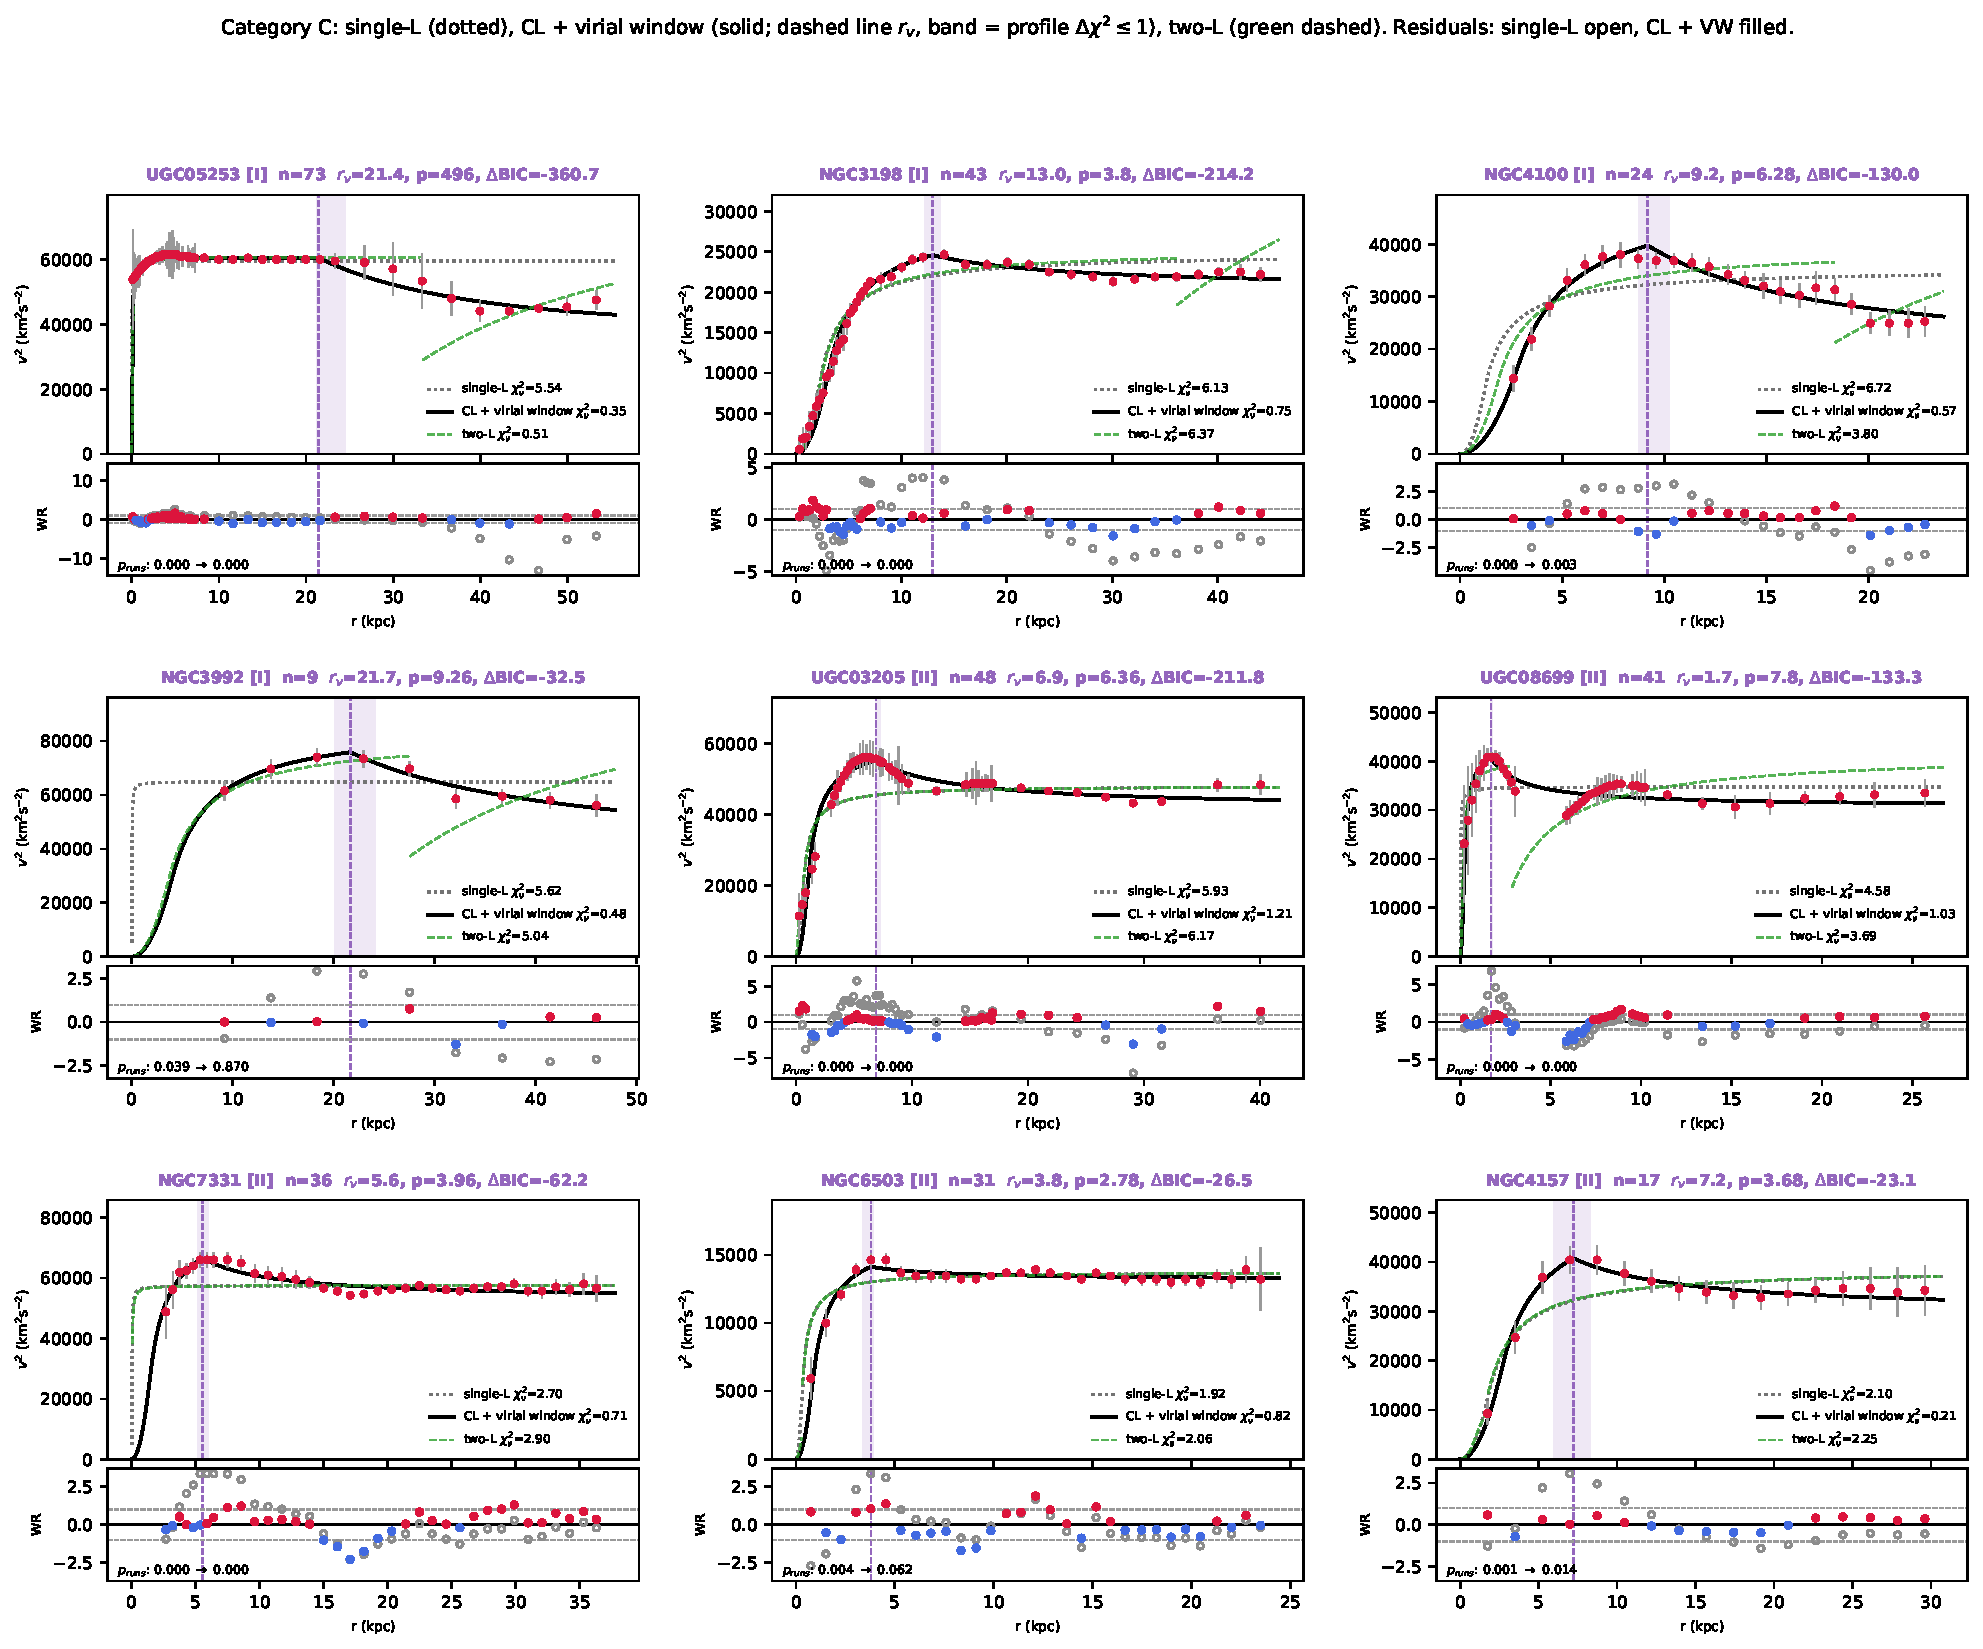
\includepdf[pages=-,landscape=true,scale=0.95]{catC_atlas.pdf}\end{document}